Quoting \href{@jwz@mastodon.social}{https://mastodon.social/@jwz}:
\url{https://mastodon.social/@jwz/111197004298988865} \#retoot

\begin{figure}
\centering
\pandocbounded{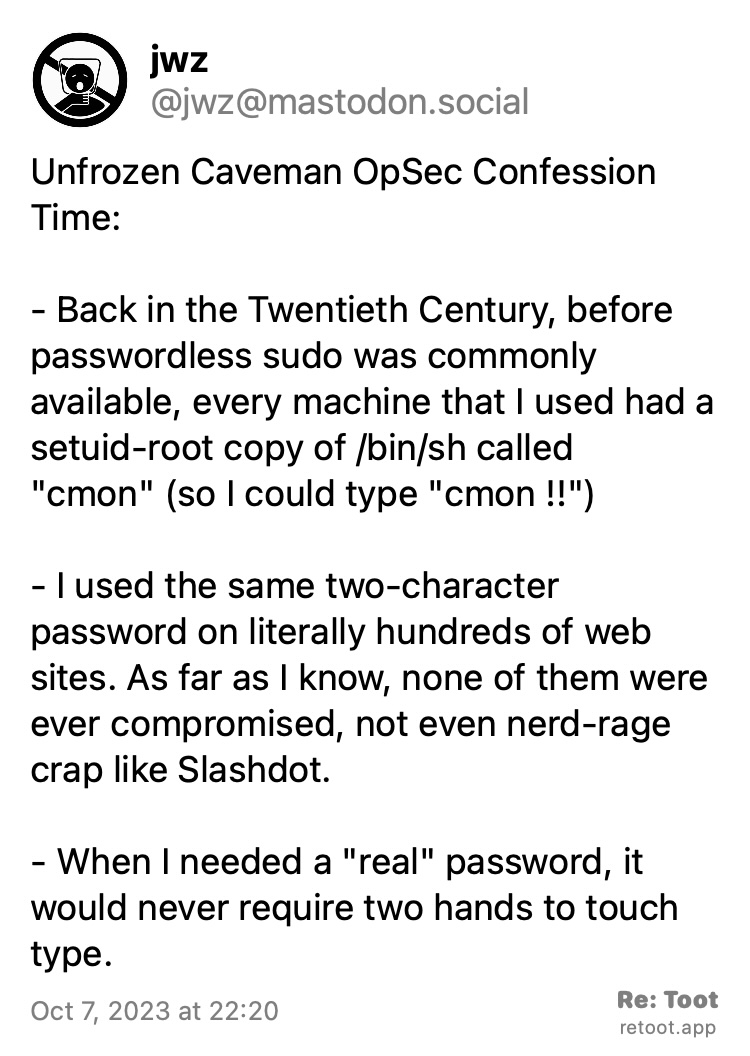
\includegraphics[keepaspectratio]{\%7B\%7Bsite.url\%7D\%7D/img/opsec.jpg}}
\caption{Post by jwz. ``Unfrozen Caveman OpSec Confession Time: - Back
in the Twentieth Century, before passwordless sudo was commonly
available, every machine that I used had a setuid-root copy of /bin/sh
called''cmon'' (so I could type ``cmon !!'') - I used the same
two-character password on literally hundreds of web sites. As far as I
know, none of them were ever compromised, not even nerd-rage crap like
Slashdot. - When I needed a ``real'' password, it would never require
two hands to touch type.'' Posted on Oct 7, 2023 at 22:20}
\end{figure}

\begin{quote}
\emph{Post by jwz. ``Unfrozen Caveman OpSec Confession Time: - Back in
the Twentieth Century, before passwordless sudo was commonly available,
every machine that I used had a setuid-root copy of /bin/sh
called''cmon'' (so I could type ``cmon !!'') - I used the same
two-character password on literally hundreds of web sites. As far as I
know, none of them were ever compromised, not even nerd-rage crap like
Slashdot. - When I needed a ``real'' password, it would never require
two hands to touch type.'' Posted on Oct 7, 2023 at 22:20}
\end{quote}

I thought I would be totally gobsmacked by this yet then I remembered
the old mainframe I used in one job. There were a ton of password
limitations because the mainframe was still in use for years after its
End of Life and I think it is still in use today. It is a miracle that
that thing remains secure.
